\documentclass{article}
\usepackage{tikz}
\usetikzlibrary{positioning}
\usetikzlibrary{shapes.geometric}
\usetikzlibrary{shapes.symbols}
\usetikzlibrary{shadows}
\usetikzlibrary{arrows}

\pagestyle{empty}

\begin{document}

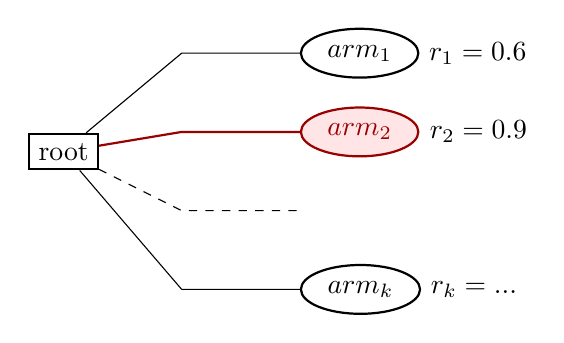
\begin{tikzpicture}
[switch/.style={shape=rectangle,draw,thick,right},
 arm/.style={shape=ellipse,draw,thick,right},
 selected/.style={draw=red!60!black},
 seledge/.style={selected,thick},
 selnode/.style={red!60!black,selected,fill=red!10!white}]

\draw (0,0) node (root) [switch] {root};

\draw (root) -- ++(1.5,1.25) -- ++(1.5, 0)
	node (a1) [arm,label=right:{$r_1=0.6$}] {$arm_1$};

\draw [seledge] (root) -- ++(1.5,0.25) -- ++(1.5, 0)
	node (a2) [arm,selnode,label=right:{$r_2=0.9$}] {$arm_2$};

\draw [dashed] (root) -- ++(1.5, -0.75) -- ++(1.5, 0);

\draw (root) -- ++(1.5,-1.75) -- ++(1.5, 0)
	node (a3) [arm,label=right:{$r_k=...$}] {$arm_k$};

\end{tikzpicture}
\end{document}
